\newcommand{\colVec}[1]{\begin{bmatrix} #1_0 \\ #1_1 \\ \vdots \\ #1_{n-1} \\ #1_{n} \end{bmatrix}}

\section{Batteries}
The basis of batteries needs an introduction. In this section, batteries and how they are designed and how they operate will be explained. A special focus will be dedicated to electrodes which are the part of the battery that this work is focused on. Some of the more essential properties related to the chemistry of the work will also be introduced. 


\myworries{ "The most advantageous combination of cathode and anode materials are those that will be lightest and give a high cell voltage and capacity. \cite{reddy2011linden}"\\
Some of the most important properties in an anode are; Hight coulombic output(Ah/g), good conductivity, stability. \\¨
Practically anodes are metalls. Li- are a good example of this, it is the lightest metal with a high value of electrochemical equivalence. With the development of intercalation electrodes, lithiated carbons are finding wide use. Lithium alloys are also being explored for use as anodes in lithium-ion battery.\\
The cathode must be a good oxidizing agent, be stable, when in contact with a electrolyte, and have a useful working voltage. }

\subsection{Cell operation principles and design}
Batteries and fuel cells are electrochemical devices. They stort chemical energy that can be converted into electrical energy. This is done by a oxidation-reduction (redox) reaction where one of the species in the reaction gain or lose an electron by changing the oxidation number. 

A battery consists of one or more \textit{cells}. A cell is composted of three parts; the anode, the cathode, and the electrolyte.

The anode is an negative electrode, which refers to the direction of current through the electrode. It is a metal that would oxidize if given the opportunity. For a conventional current flow the electron moves from the anode to the cathode. The anode is normally low voltage.  

The cathode is a positive electrode. The cathode is a metal that is normally combined with oxygen and is where the reduction occurs. A common example of a oxide is iron oxide, this oxide is very fragile, but their are oxides that are strong enough to be shaped before used in the cell. The cathode is normally high voltage. 

The electrolyte is the material that, when introduced to the anode and the cathode, provides an electrically conducting medium for transfer of charge. The anode draws oxygen atoms toward it, creating an electrical flow, with electrons moving from the end of the anode to the end of the cathode not emerged in the electrolyte. The electrolyte is typically a liquid, to impart ionic conductivity. It is often alkaline and when this is the case the battery is a alkaline battery. It can be a solid, but this is less common. The cell will not produce electricity without a circuit that is complete. The electrolyte can, in some designes, act as both the electrolyte and the anode or cathode. If the anode is made from pure metal and has an external cathode of ambient air it is referred to as a metal-air electrochemical cell. These batteries have a much higher theoretical energy density. However there are technical issues confronting their development. \cite{li2017metal}


The difference between high- and low voltage is referred to as the cell voltage, which is the driving force for the discharge of the battery. For secondary batteries, as are the one in question (\myworries{Not really true, we are only looking at Electrodes.}), it is possible to recharge batteries by reversing this process by applying an external electrical power source, so that it creates a over-potential - a higher voltage than the one produced by the cell, with the same polarity. 

Changes in the design of the cell dictates the cells performance. If the compositions of the anode and cathode are changed, the cell will yield more or less electricity. Adjustments in the cell can affect the amount of electricity, the rate of production, the voltage, and the cell's ability to function in different temperatures. There is almost an endless amount of possibilities, even though the most common cell has been $1.5$ volt alkaline batteries. Other types of batteries include Lithium  batteries, Magnesium batteries, Zinc batteries,  Mercury batteries and others. \myworries{Should cover these shorty in another subsection? Write something about Magnesium and Li- as a minimum.}

\subsubsection{The manufacturing process of an Alkaline battery}
In alkaline batteries the cathode is used both as the container and the cathode. Manganese dioxide, graphite, and the electrolyte are mixed and ganulated and pressed into hollow cylinders called preforms. The preforms can be stacked or replaced by an extruded ring of the same material. The preforms are then combined with nickel-plated steal. These are then the containers of the battery. 

A separator is then soaked in the electrolyte solution and inserted between the cathode and where the anode is supposed to be. The anode is then put into the can, in a Alkaline battery like this, it is a gel composed of zinc powder and other materials like potassium hydroxide electrolyte. The gel does not fill the whole can, so that their is room for the chemical reaction to occur. 

The can is then sealed with three connected components. The first being a current collector, going to thirds of the way trough the anode with a plastic seal at the top before it is all closed by a metal cover with a metal cap. The current collector goes all the way through the plastic seal and is connected to the metal cap. The seal is thinner in some places, in case of gas build ups. In some battery designes, wax are used instead of a plastic seal, so excessive gas can push through the wall. Lastly a label is attached to the battery, with the necessary information about the battery. 

The battery is then take through a complex quality control, to certify the batteries ability to resist corrosion, maintain a good shelf life, usage life, and other factors. 

\myworries{useless section?}




\subsubsection{Theoretical Cell voltage, Capacity, specific Energy, Energy density}\label{sec:msp}
	
	In a cell there are essentially two areas or sites in the device where the redox reactions occur. In general these half-cell reactions can be expressed as one reduction and one oxidation reaction:
	
	$$aA + ne \leftrightharpoons cC $$
	
	where a is the number of molecules of substans A taken up by n electrons to form c molecules of C, and the oxidation reaction defined in the same way:
	
	$$bB \leftrightharpoons dD + ne $$ 
	
	with the overall reaction being: 
	\begin{equation}
	aA + bB \leftrightharpoons cC+ dD
	\label{eq:redox}
	\end{equation}
	
	Whenever there is a reaction, there is a decrease in the free energy of the system, namely standard Gibbs energy, and is defined as:  
	
	$$\Delta G^0 = -nFE^0$$
	
	Where $n$ is the number of electrons in the reaction, and $F$ is the Faraday constant. 
	
	$E^0$ is the standard potential of the cell is determined by the type of active material in the cell, and can be calculated from the free energy. The standard potential of a cell can be calculated form the standard electrode potential.
	
	$$\text{Anode} + \text{cathode} = \text{standard potential}$$ 
	
	\myworries{example?}
	
	In the situation where we are not in the standard state, the voltage $E$ of a cell is given by the Nernst equation.
	
	$$ E = E^0 -\frac{RT}{nF} \ln{\frac{a^c_C a^d_D} {a^a_A a^b_B} } $$ 
	where $a_i$ is the activity of the species. $R$ is the gas constant, and $T$ is the absolute temperature. 
	
	Gibbs free energy of the reaction is the driving force of the battery, and enables it to deliver energy to an external circuit. 
	
	
	The theoretical \textit{capacity} is determined by the amount of active material in the cell. If the calculation are based on only the  active materials participating in the electrochemical reaction the theoretical capacity of a $\ce{Zn/Cl_2}$ cell is $0.394 \si{Ah/g}$
	
	$$\ce{Ze} + \ce{Cl_2} \rightarrow \ce{ZnCl_2}$$
	$$1.22 \si{g/Ah} + 1.32 \si{g/Ah} = 2.54 \si{g/Ah}$$
	
	Capacity can be defined as:
	\begin{equation}
	C = \int I(t)\cdot dt
	\end{equation}
	
	And is the $i$ number of electrons or cations exchanged between the negative and positive electrodes. $I(t)$ is the current, i.e. the number of electrons flowing over the external circuit per time interval $dt$ which is integrated over the discharge period. The capacity is normally expressed as $\si{Ah/kg}$. Theoretically, 1 gram equivalent weights of the active material in grams divided by the number of electrons in the reaction.
		
	The battery can deliver a power that is defined as
	\begin{equation}
	P(t)=V(t)I(t)
	\end{equation}
	Where $I(t)$ is defined as earlier, and drawn at a cell voltage $V(t)$. The amount of work that can be done by the battery, or; the energy contained in the battery, is then defined as the power delivered over the discharge period
	\begin{equation}
	W = \int P(t) \cdot dt = \int V(t)I(t) \cdot dt
	\end{equation}
	
	Specific capacity and energy densities of battery materials can be compared relative to mass, volume and cost. The more electrode material that a battery contains, the greater is its capacity and energy. The higher the cell voltage the greater its power and energy. 
	
	The active materials of the electrodes allow the reversible uptake and release of Mg, or Li ions. This may happen by; movement of the  ions; into, i.e. \textit{intersection} or \textit{intercalation} or out of, i.e. \textit{extraction} or \textit{deintercalation}, their chemical structures, \textit{phases}. This is done by conversion of the materials between ion poor and rich i.e. \textit{alloying}, or rich and poor, e.g. \textit{dealloying} phases, this can also be done by conversion of the electrode material into other more ion rich/poor chemical forms or mixtures. Referred to as \textit{conversion} or \textit{displacement} reaction, with the average ion content of the entire electrode varying. 
	
	The total Li or Mg content in the electrodes will thus either be varied by changing the composition of one phase or the ratio between coexisting phases. In this work \myworries{?}we will only look at \textit{intercalation} type batteries, due to the \textit{database}, more on this later.
	
	\subsubsection*{Specific Energy}
	Specific Energy, or gravimetric energy density, defines battery capacity in weight, energy density, or volumetric energy density, defined as: 
	\begin{equation}
	\text{Watthours/gram} = \text{Voltage} \cross \text{Ampere-hours/gram}
	\end{equation}	
	
	


\subsection{Cell limitations \& definitions }
In this paper, especially under the section on general properties of battery, an amount of technical terms related to material details, from  is used. Here I will clarify what we mean by these terms. 

	
	
	\subsubsection{Polarization}
	Polarizability is a tabulated atomic properties, it is the ability to form instantaneous dipoles(REF), and is defined as: 
	
	$$	\alpha = \frac{P}{E}	$$
	
	Where $\alpha $ is the polarizability in isotropic media, $p$ is the induced dipole moment of an atom to the electric field $E$ that, is the field that produces the dipole momentum. 
	
 



		



\subsection{Battery chemistries}

\subsection{Intercalation batteries and why Li}

"Among the rechargeable battery technologies (Fig. 11
), the
current Li-ion battery technology offers the best useable energy
and tap density, dominating the worldwide market for mobile
electronic devices2 for decades. Li-ion batteries have minimal
(unwanted) side reactions when a Li ion intercalates into or
desorbs from the cathode/anode materials. Their energy efficiency
may be further enhanced by lowering the internal resistance of the
battery, and they exhibit limited self-discharge, and no memory
effects that limit energy density after many cycles. Li-ion batteries
as a result, receive considerable attention at both fundamental and
applied research levels.


The development
of stable novel materials is the key to the success of development
of novel and advanced rechargeable batteries. Current research
and development has focused on upgrading the energy density
of Li-ion batteries. 

Most practical
rechargeable batteries deliver capacities and energy densities
far below their theoretical values(med kilder)due to limited utilization
efficiency of the active materials that participate in electrochemical reactions. The major reasons for such limitations
include effects that result from slow electrode process kinetics
with high polarization and low ionic diffusion or electronic
conductivity rates, particularly at the electrolyte–electrode interfaces. Material stability issues caused by a low Li content can
also impact on its degree of charging. Therefore, the improvement
in existing rechargeable battery systems involves exploring key
materials and focusing our attention on the atomic, ionic, or
molecular diffusion and transport. Charge transfer, the optimization of surface and interface structure, and the regulation of
electrochemical reactions within Li-ion systems may pave the
way for improved (i) capacity, and energy and power density,
(ii) reactivity, reversibility, and structural stability during charge–
discharge cycles, (iii) ionic diffusion and electronic transfer at
high charge–discharge rate, and (iv) lower cost, increased safety
and environmental compatibility


inkluder litt om dette? og med bilder kanskje?

The schematic diagram of the current Li-ion battery based on
a carbon based anode (LixC6), cathode (LiCoO2), liquid electrolyte (LiPF6 dissolved in a mixture of EC and DMC or equivalent),
and separator is shown in Fig. 2.9 In the foreseeable future,
Li-ion batteries will be the most practical solution to a wide
range of electrical energy storage applications.10


. The majority new cathode
materials for Li-ion batteries under research and development
are transition metal oxides, which tend to provide lower discharge
potential as the electric-capacity density increases. Carbon-based
materials (usually graphite) are currently used as anode materials
in Li-ion batteries. The other variety of carbon-based materials and
pure Li metal are currently proposed as alternate anode materials,
but many need further improvement with respect to electrode
potential and charge–discharge cycle life concerns

"\cite{bhatt2015recent}

Working principle of Li-ion cell. 

When a Li-ion battery discharges, a $\ce{Li^+}$ moves from the anode (i.e. graphite) to the cathode (i.e. \ce{LiMO_2} where $\ce{M}$ is a transition metal), through the electrolyte that commonly is  $\ce{Li^+}$ -containing salt. The reaction, as discussed above \ref{eq:redox}, are:


$$\ce{LiMO_2} \leftrightharpoons   \ce{Li_{1-x}MO_2} + \ce{xLi^+} + \ce {xe^-}\text{ (cathode)} $$
$$\ce{xLi+} + \ce{xe^-} + \ce{xC_6} \leftrightharpoons  \ce{xLiC_6} \text{ (anode)} $$
The overall reaction:
$$\ce{LiMO_2} + \ce{6C} \leftrightharpoons  \ce{Li_{1-x}MO_2} +  \ce{xLiC_6}$$

The anode is graphite, thus there is noe metallic $\ce{Li}$, which makes the Li-ion battery less reactive, therefor safer, and the graphite anode offers a longer cycle life than their Li-metal counterpart. To progress the performance of Li-ion batteries a few design changes are needed; A cathode with a chemical potential that matches the electrolytes highest occupied molecular orbital, and an anode matching the lowest unoccupied molecular orbital of the electrolyte. A non-aqueous electrolyte of high $\ce{Li^+} $ ion conductivity under practical temperatures. 


\subsection{Electrodes and features}
	In this section the features used in ML as predictors will be introduces. First will the pair properties be introduced, before going into the more electrode specific features. 

	As a general note. These features are based on optimal design and discharge conditions. These values are helpful to set a number on the "goodness" of a battery, the actual performance may vary under normal conditions of use. \myworries{Nice to give this note?}

	
	\subsubsection*{Average Voltage}
	The theoretical voltage and capacity of a cell are function of the anode and cathode materials, with the composition of the electrolyte, and the temperature, normally $25^\circ\si{C}$.
	
	The active materials contained in the cell determines the standard potential, $E^0$, which can be calculated from the free-energy. 
	The standard potential of a cell can be calculated from the standard electrode potential:
	\begin{equation}
	\text{Anode(oxidation potential)} + \text{cathode (reduction potential)} = \text{standard cell potential}
	\end{equation}  
	The cell voltage is also dependent on other factors including concentration and temperature, as expressed om the nernst equation. (REF)
	\textit{Average Voltage} as we use, is defined as the voltage average during the discharge. It is lower then the theoretical voltage.

	 


	\subsubsection*{Physical stability}
	What we refer to as Physical stability is Energy above hull. The energy that is demanded for decomposition of the material into the set of most stable materials at that chemical composition. Some positive value indicates that the material is not stable. While a zero energy above hull indicates that this is the most stable material at its composition. 
	
	\subsubsection{Properties of materials}
	Are These (or some of them) theoretically computed properties. If yes provide some details about how they computed (i.e. DFT methods)

Total \textit{Magnetic Moment} ($\si{\mu_B}$) is calculated for the unit cell within the magnetic ordering provided. 


The \textit{Formation Energy per Atom} is calculated from the formation energy from the elements normalized to per atom in the unit cell.

\textit{Energy Above Hull per Atom}
The energy of decomposition of the material into the set of most stable materials at this chemical composition, in $eV$ per atom. Stability is tested against all potential chemical combinations that result in the material's composition. For example a $\ce{Mg_3Sb_2}$ structure would be tested against other $\ce{Mg_3Sb_2}$ structures, against $\ce{Mg}$ and $\ce{Sb}$ mixtures, and against $\ce{MgSb}$ and $\ce{Sb_2}$ mixtures. 

\textit{Density}, here defined as the calculated bulk crystalline density, typically underestimated due to the calculated cell volume being overestimated on average by $3\% (+\/- 6\%)$.

The \textit{Band Gap}s are calculated a little different. In general, band gaps are computed with common exchange-correlation functionals such as the LDA \cite{perdew1983physical} and GGA are severely underestimated \cite{perdew1985density}. Typically the disagreement is reported to be $\tilde 50\%$ in the literature. Some internal testing by the Material Project supports these statements; typically, they found that band gaps are underestimated by $\tilde40\%$. We additionally find that several known insulators are predicted to be metallic. 
	
	\subsubsection*{Cycle life}
	
	

	\subsubsection*{Rate capability}
	RC
	\subsubsection*{Self discharge}
	SD
	\subsubsection*{Energy per atom}
	EpA
	\subsubsection*{volume}
	Volume of the unit cell defined as 
	
	\subsubsection*{Formation energy per atom}
	Fepa
	\subsubsection*{Band gap}
	The band gaps of a solid is simply the range of energies an electrode in a solid can not have. While the bandstructurs.
	\myworries{How much to include? Should I here have a page on quantum physics and the bandstructure? - Only include relevant stuff.}
	
	\subsubsection*{Total magnetization}
	Tm
	\subsubsection*{Elasticity}
	E
	\subsubsection*{Porous Electrodes}
	In a fuel cell system, the reactant is supplied from the electrolyte phase toe the catalytic electrode surface. Electrodes are often composites made of active reactants, binders and fillers, in batteries. To minimize the energy loss of both activation and concentration polarizations at the electrode surface and to increase the electrode efficiency or utilization, it is often preferd to have a large electrode surface area. This can be done by have a porous electrode design. A porous design can provide an interfacial area per unit volume that is considerable higher den that of a planar electrode. 
	
	A porous electrode is a electrode that concists of porous matrice of solids and void space. The electrolyte penetrates the void space of a porous matrix. In such an active porous mass, the mass transfer condition in conjunction with the electrochemical reaction occuriing at the interface is very complicated. In a given time druing cell operation, the rate of reaction within the pores may vary significantly depending on the location. The distribution of current density within the porous electrode depends on the physical structure(pore size), the conductivity of the solid matrix and the electrolyte, and the electrochemical kinetic parameters of the electrochemical processes.  
	

\subsection{On Mg- and Li- batteries and their state today}
	
	
	
\pagebreak
\section{Machine Learning}

In this chapter we summarize some concepts of machine learning and related ideas. The first section introduces the basic ideas behind machine learning and *some of the best known examples* will be presented. Secondly the concepts of supervised and unsupervised learning will be presented with a clarification on the difference between regression and classification problems, so that we can define where in the field of machine learning this work resides in. Basics of methods utilized in this work will be introduced, emphasizing Random forest. Subsequently a short description of the validation methods used is given. These are; K-fold cross validation and how it is used in optimizing our random forest method, mean square error(\textit{MSE}), root mean square error (\textit{RMSE}) and R-squared($R^2$). 
   
Before we round of this section with a brief explanation on the role of data, how features can affect the effectiveness of a model, and finalizing with the concepts of over- and under-fitting, and how these are related to the bias-variance-trade-off. 


\myworries{Sondre: Did you forget something? Come back to this when done with the section.}


\subsection{The basics of Machine Learning}

Machine learning comes from the field of pattern recognition and learning theory, and is defined as the field of study that gives computers the ability to learn without being explicitly programmed. Or more precise: "… A computer program is said to learn from experience E with respect to some class of tasks T and performance measure P, if its performance at tasks in T, as measured by P, improves with the experience E…"(\cite{mitchell1997machine}). At its core the ability to learn by detecting patterns in usually huge amounts of data that, more often then not, is impossible to perceive for a human. 


	\subsubsection{Example time!}
	As an introduction on how machine learning was applied to learn and recognize patterns in our work, it will be useful to start with a simple example applied to the recognition of the handwritten number "5". (PICTURE TIME!)
	
	How two people writes a single digit may vary to an extensive degree. It might seem to be a easy problem, but if the recognition is to be done manually million of times, it is no longer a trivial task for any one human being. Therefore a model which can recognize these digits would be useful. A model that takes a picture of a digit and outputs that digit in a way that is recognizable for a machine, that is, a digital format.
	
	Machine learning only works when you have data, preferably a large amount of data. For instance data from the MNIST test dataset(\cite{lecun1998gradient}). This database contain $60,000$ images of handwritten numbers that is commonly used for both various training, and testing in the field of machine learning. The images all are 18x18 pixels. The data is divided into two sets, one training set: $X_{Train}$ and one test set: $X_{test}$
	
	How do one represent an image as something that makes logical sense to a computer? Most learning algorithms take numbers as input. To a computer one image is nothing more than a grid of numbers that represent how dark a pixel is. So each picture contains a gray-scale value that ranges from $0$ to $255$. Where each sample can be viewed as a vector consisting of 324 \textit{features}. Every sample has a corresponding label value, or \textit{target}, which is the digital equivalent to the handwritten sample. We let the corresponding targets be denoted: $Y_{train}$ and $Y_{test}$, for training and testing data. Next we designate our \textit{learner} denoted by function A. A is then given our training set $S$, where $S = (X_{train1}, Y_{train2}),..., (X_{trainN}, Y_{trainN})$ and returns a prediction rule: $h: X \rightarrow Y$. This rule is also called a predictor, in general, a classifier, or a regressor, depending on the problem in question. 
	
	The \textit{training phase} is a prosess where the learning algorithm gets tweaked to best capture the correlating structure of the data set, so that it can better predict new data. As mentioned in the last paragraph the output from the \textit{training phase} is called a \textit{predictor}. The next step is to introduce the \textit{predictor} for new, unseen data, so that it can be classified. Then we compare the $Y_{test}$ to our predicted value $Y_{pred}$ given by $h$ to see if our model generalizes well to unseen data in $X_{test}$. 
	
	\subsubsection{Supervised and Unsupervised Learning }
	One of the most basic separations in machine learning is the partition between supervised learning and unsupervised learning. \cite{gentle2012handbook}
	
	In the case of supervised learning one knows the answer to a problem, and let the computer deduce its own logic to figure out how we get to that result, thus the name complete-date problem is commonly used. This is the most common type of learning. With unsupervised learning the machine is tasked with finding patterns and relationships in data sets without any prior knowledge of the system, incomplete-data problems. Some authors operate with a third and a forth category, namely reinforcement learning, where the machine learns by trial-and-error(marsland2014machine), and evolutionary learning, where they account for the biological evolution and that it can be seen as a learning process.
		
	In this thesis we only consider supervised learning. Algorithms and challenges specifically related to unsupervised learning, reinforcement learning, and evolutionary learning, is therefore not further examined. 

	\subsubsection{Regression and Classification Problems}
		A respons variable can either be qualitative or quantitative in nature. For the qualitative respons variable, let's assume a set of data points $ \vec{x}$ and a goal of finding the value of the output $y$ when $x = 0.5$. The value $x = 0.5$ is not in the data points given so it is needed a way to \textit{predict} the value. Given in the example above, we assume that there exists a function $h$ that the value comes from. When that function is found one can find any given $y$ for any given $x$. This is what is known as a regression problem - The respons takes form of a continuous numerical value. The regression problem is a problem of function approximation or interpolation. It may occur a scenario where there are multiple functions, lets say $h$ and $g$, that fits the given data perfectly. If this is the case one need to pick a value in between our data points and use our functions $h$ and $g$ to predict its values and compere the result to see which is better. \myworries{mby connect it tighter with the handwritten example?}
	This does not seems as very intelligent behavior, but the problems of interpolation can be very difficult in higher dimensional space. This will also be observed in classification, the other aspect of what our algorithms can do.  
	
	If the response variable is quantitative the problem is referred to as a classification problem. Such a problem consists of taking several input vectors and deciding which of $N$ classes they belong to. This decision or prediction comes from training on examples of each class. I underline again that classification problems are of a discrete nature - The input only belongs to one class.
	
	In this work we want to predict characteristics of batteries , meaning  that our task is a regression problem.
	
	\subsubsection{Data collection, Preparation, Features and Feature Selection}
	 
	Normally the data collection is a enormous part of the work and not easily available, or, at the very least, needs to be assembled and prepared. If the problem is completely new it might be natural to engulf this step with the next one. (Which is, more or less, what this work tries to do.) With a small dataset with many different features one can experiment and try to figure out what features are the most useful before picking those and collecting a full dataset based on them before doing a complete analysis. 
	
	A common problem is that there is too much data that can be relevant, but that data is hard to find or represent in a way that makes sense for the machine. This can be because it requires too many measurements, or, something thing that is prevalent in this work\myworries{(How much should I refer to this here and not later?)}, that they are in a variety of places and formats. For instance; if the measurements are already taken, but at vastly different temperatures they might be hard to compare or merge. It is important to have a \textit{clean} dataset, this means that the dataset does not have missing data, significant errors, and so on. On top of all of this, supervised learning requires a target $y$, which demands time and involvement of experts. 
	
	The specific input to a model is normally referred to as a feature, that is, numerical representation of raw data. The amount of features are of importance for the machine learning algorithm to successfully make a good prediction. If there are to few relevant features one can not make an accurate prediction due to the lack of necessary data. And if there are to many features, or many of the features are irrelevant to the task the model will be more expensive.
	
	The amount of information needed is extensive, and should be of high quality. A bigger dataset demands a higher cost, and predicting the amount of data required is a futile endeavor. Luckily Machine Learning is still less computationally costly than modeling full systems at a micro or nanoscale, which makes it interesting in the field of material science. 
	
	
\subsection{Bias-variance tradeoff}\label{sec:Bias-variance tradeoff}

As the algorithm learns we need to make sure that it generalizes well to data not in our training set. Obviously the algorithm can not generalize beyond the limits of the training data. Therefore it is important to minimize the two sources of errors known as \textit{bias} and \textit{variance}. This is know as the \textit{bias-variance trade off}. It is the property of trying to minimize the two errors simultaneously, and should not be confused with the \textit{irreducible error} of a model which is a result of the noise of the data. These three together are the terms used to analyze an algorithms expected \textit{generalization error}, which will be handled later(Ref).    

\begin{figure}[H]
     \centering
     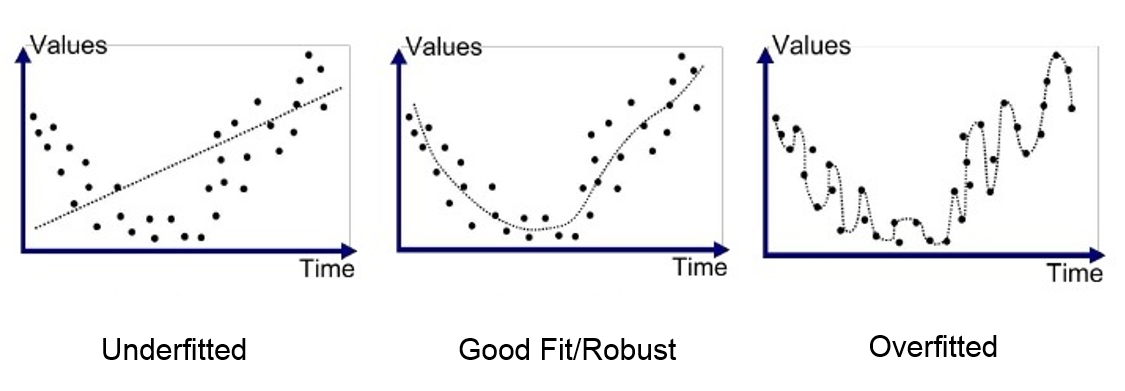
\includegraphics[width=\linewidth]{theory/figures/Bias_variance.png}
     \caption{Simplified illustration showing the concepts of bias-variance problem. Left to right; high bias, low bias and low variance, high variance. Adopted from \cite{fig:bias_var}}
     \label{fig:bias_var}
\end{figure}
Our machine is bias if it generalizes to much. The error is due to low variability in our training data, or that it did not adapt to the training data appropriately. The machine misses the relevant relations in the data set between the features and the output. This effect leads to that which is commonly referred to as under-fitting, see left on figure \ref{fig:bias_var}. 

Variance is the error that stems from high variability, and the number of degrees of variability in most machine learning algorithms is huge(\cite{marsland2014machine}). In simple terms there is a low degree of generalization. It might be a perfect fit, but as soon as new data is introduces our predictions plummet. This is commonly referred to as over-fitting, see right on figure \ref{fig:bias_var}. 

A good way to understand the idea of bias-variance tradeoff is that a more complex model with an increased number of features is not necessarily better at predicting what you want to predict. 


\subsection{Random Forest}

\myworries{Should I use more math? I am trying to expaine these things as simple as possible with little mathematical syntax}	

\subsubsection{Ensemble learning}
	There are many different machine learning algorithms, in this work we have focused on the \textit{ensemble method}; \textit{Random forest}\cite{breiman2001random}. The idea of ensemble learning is that two heads are better than one, so why not have many learners that all get slightly different results on the same data, and then combine them.  
	
\begin{figure}[H]
     \centering
     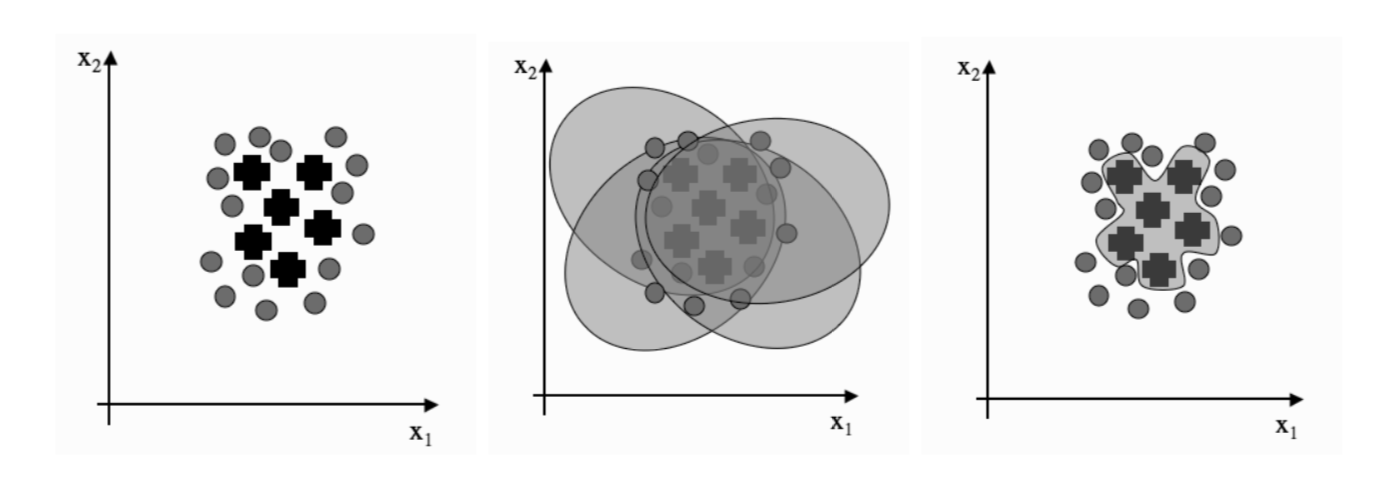
\includegraphics[width=\linewidth]{theory/figures/ensemble_learning.png}
     \caption{Combining a lot of different classifiers trained on the same data, which in combination can make a much better decision boundary on the target data. Adopted from \cite{marsland2014machine}}
     \label{fig:ensemble_learning}
\end{figure}	

Ensemble methods are particularly usefull in machine learning when there is little data, as well as when there is much data, this is heavily due to cross-validation, see(Ref to other section on cross-validation). 

\subsubsection{Decision tree}

A decision tree is a low cost binary flowchart-like structure. It is one of the most common data structures in the field of computational science, both because of the low cost to make the tree, but also because the cost of using the tree is even lower; $\mathcal{O}(\log{N}$, where N is the number of datapoints.\cite{marsland2014machine}. 

Decision trees are structured much like a regular tree\ref{fig:decision_tree}; at the top there is a base, or a \textit{root}, down the branches there are chance nodes, and at the end of the branches there are \textit{leaves}, or end nodes. Every internal node is structured like an conditional statement on a feature.\myworries{Example? If overcast, play. Rain -> more questions} The chance nodes are the results from these tests, and the leaves are the class labels. The full route from root to leaf is the classification rule. An advantage of random forest being based in decision trees is that the algorithm is much more like a "white box" compared to Neural networks black box approach, because we can retrace the decisions of each tree. This is especially helpful in the research done in this work where we want to figure out the roll of every feature, and how they affect the result.

\begin{figure}
\begin{tikzpicture}
  [
    grow                    = right,
    sibling distance        = 6em,
    level distance          = 10em,
    edge from parent/.style = {draw, -latex},
    every node/.style       = {font=\footnotesize},
    sloped
  ]
  \node [root] {Outlook}  
    child { node [dummy] {Humidity}
      child { node  [env] {No} 
        edge from parent node [below] {High}}
	  child  { node  [env] {Yes}  
	  edge from parent node [below] {Normal}}
	  edge from parent node [below]{Sunny?}}
%  --------------------------------------------------------  
    child { node [env] {Yes}
      edge from parent node [below] {Overcast?} }
%  --------------------------------------------------------    
    child { node [dummy] {Wind}
      child { node  [env] {No} 
        edge from parent node [below] {Strong}}
	  child  { node  [env] {Yes}  
	  edge from parent node [below] {Weak}}
	  edge from parent node [below]{Rain?}};
\end{tikzpicture}
\caption{A simple example of a decision tree for playing tennis. Root in red, leaf node in blue. Adapted from \cite{fig:decision_tree}}
\label{fig:decision_tree}
\end{figure}



\subsubsection{Random forest}
Random forest is ensamble such a learning method, the idea is that one decision tree is good and many trees, or a forest, is better. The most interesting part of random forest is the randomness that is introduces. Several classifiers are achieved by using the simple combination method \textit{bagging}. Bagging stands for \textit{bootstrap} aggregating. Bootstrapping is the process of taking a sample from the original dataset at random, and replacing parts of it with other original data, so that it is not equal to the original data. There will then be several samples where some of the data is equal, while others are completely different. For the bootstrapping in random forest, one sample is taken from the dataset for each tree. 

Then a new parameter is introduced, at each node a random subset of features are given to the tree, and it can only make decisions based on that specific subset, and not the original tree. This increases the randomness in the creation of each tree, and it speeds up the learning process. The reason to add randomness to the algorithm is to reduce variance without effecting bias. It also removes the need for decision tree \textit{pruning}, that is, reducing the complexity of decision tree by removing the parts of the tree that does not help the classifier. This reduces overfitting. The process of creating trees is repeated until the error stops decreasing. 

When the forest is done, we use a majority vote system, which is a comparison of the mean response for regression. For a point by point algorithm, see the appendix(REF to appendix). 
The reason for not using cross-validation in the learning algorithm, which is common in other machine learning methods (Ref to cross-val), is that our bootstrap method only uses about $65\%$ of the data, leaving $35\%$ on average which can give a estimated test error. 

The main reason we decided to opt in for random forest is due to an article by .... that clearly states that random forest is the go to machine learning algorithm when you are not sure where to start. 


%\subsection{Support Vector Regression}
%	Dette bør brukes og kan da skrives om.
%	\subsubsection{Radial Basis Function Kernel}
%	\subsubsection{SVR and the Bias-Variance-Trade-off}
	
	

\subsection{Mean square error and Root mean square deviation}
The Mean Square Error (\textit{MSE}) can give a measure of the quality of our estimator.(ref) It is defined as
\begin{equation}\label{eq: mse}
	\textit{MSE}(\epsilon) = \frac{1}{n}\sum_n^{n-1}\epsilon^2 = \frac{1}{n_\text{samples}} \sum_n^{n_{\text{samples}}-1}(y_i - \hat{y_i})^2
	\end{equation}
	Where $\hat{y_i}$ is the predicted value of the $i$-th sample, and $y_i$ is the corresponding true value.
As such it can be thought of  as the average of the square of our residuals. Therefore the \textit{MSE} can never have negative values, and smaller values mean that we have a better prediction, where at zero there is a perfect fit.

The Root mean square deviation, or root mean square Error(\textit{RSME}), is the squared for the MSE:
$$RMSE = \sqrt{MSE} =  \sqrt{\frac{\sum^{n-1}_{n}(y_{i}-\hat{y_{i}})^2 }{n}} $$
And is thus the distance, on average, of a data point from the fitted line, measured along a vertical line. The \textit{RSME} is directly interpretable in terms of measurement units, and so is a better measure of goodness of fit than a correlation coefficient. 

\subsection{$R^2$ score - The Coefficient of Variation}

	In regression validation the $R^2$ is the standard when it comes to measuring goodness of fit.(\cite{coef} \myworries{Needs new ref.}) In straight terms it is the proportion of the variance in the dependent variable that is predictable from the independent variable (S).

\begin{equation}\label{eq: R squared}
	R^2 =1 - \frac{SS_{res}}{SS_{tot}} =  1 - \frac{ \sum(y_i-f_i)^2 }{ \sum(y_i-\bar{y}_i)^2 }
\end{equation}

	Where $y_i$ are the indexed response variables (data  to be fitted) and $f_i$ the predictor variables from the model with $\epsilon_i = y_i - f_i$. The average of the response variables is denoted $\bar{y}_i$. The second term can also be considered as the ratio of \textit{MSE} to the variance (the $1/n$ factors null each other out in a fraction), or the total sum of squares (\textit{SS\textsubscript{tot}}). 
	
	If the residual sum of squares (\textit{SS\textsubscript{res}}) is low the fit is good. However, this should be compared to the spread of the response variables. After all, if the response variables are all nicely distributed close to the mean, then getting a good \textit{SS\textsubscript{res}} is not suspicious. We therefore do a normalization in the fraction, taking the scale of data into consideration. In the simplest polynomial fit, using a zero order polynomial (a constant), our model would just be a constant function of the mean. The sums being equal, returning unity on the fraction and the total $R^2$ score would be zero. In the other extreme, if the model fits perfectly, then \textit{SS\textsubscript{res}} would be zero and the $R^2$ score would be one. In this sense we have a span of possible $R^2$ scores between zero and one, from the baseline of the simplest model at zero, and a perfect fit at one. In contradiction to most scores the value can be negative, because the model can get arbitrarily worse, thus giving negative values.
	The $R^2$ score is useful as a measure of how good our model is at predicting future samples.
	 

\subsection{Principle Component Analysis }
	Principle Component Analysis(\textit{PCA}) is a procedure that uses orthogonal linear transformation to reduces the amount of feature subspaces. It goes under different names in different fields, but the most recognizable might be Singel Value Decomposition. This is done by converting a set of possible correlated variables into a set of uncorrelated variables, called principle components(\textit{PC}). 
	
	The \textit{PC} are arrange so that the first \textit{PC} has the largest variance, meaning that it accounts for as much of the variability in the data given as possible. The next \textit{PC} does the same, it accounts for as much of the variability as possible with the constraint that it is orthogonal to all the former components. These orthogonal vectors are linear combinations being an uncorrelated orthogonal basis set. Graphically the shortest vectors effects the predictions the least. \textit{PCA} is sensitive to the relative scaling of the original variables, so in \textit{sklearn.decomposition.PCA} the input data is centered but not scaled for each feature before the SVD of the date is applied. 

\subsection{K-fold cross validation}
	K-folding is a cross validation technique that allows us to generalize the trends in our data set to an independent data set. In this way we can circumvent typical problems like over-fitting and selection bias.(ref=\cite{cross-valid} )The approach for the technique is simple. Instead of doing a regression on the entire data set, it is first segmented into $k$ number of subsets of equal size (making sure to pick out the variables randomly before distributing them to the subsets). 
	
	Now one subset can be chosen to be the 'control' or 'validation' set while the rest of the subsets are the training sets. The desirable regression is then applied on the training set, arriving at some data fitting that is the prediction. From here it is a straight forward process to analyze how well our predicted variables compare to the validation variables, for example through the $R^2$ score function. However, even though the subsets are picked randomly, the validation subset used could potentially not be a representative selection of the entire set. Therefore the process is repeated \textit{k} times, each time using a new subset as the validation subset. After all this is done one can simply calculate the average of the scores to get the predictive power of our model. As an added benefit, since the calculations are done anyways, the average of the predictions can be used as the final fit. 
	
	Cross validation techniques are extremely useful when the gathering of new data is difficult or, sometimes, even impossible, as we are using the extra computational power at our disposal to squeeze the most amount of relevant information out of our data.\\

FIGURE?
link to good crossvalidation.
\url{https://scikit-learn.org/stable/modules/cross_validation.html#cross-validation}

\subsection{Mutual Information**}
Ranking of features. 
This can be useful.

\subsection{Machine Learning $\cross$ batteries}
State of the art.
What has been done in this field? 
Similar predictions of the kind we are interested in, have been done by 
Sandek: \cite{sendek2017holistic}


















%------------------------------------------------------------------------------------------------
\begin{comment}
\section{Batteries}
Basic principles behind batteries, as well as some critical battery characteristics or specifications, including battery voltage, capacity, charging/dischargning regimes, efficiency, and more.

Theoretical energy: Watthours per kilogram (Wh/k) is specific energy, on a volume basis. Watthour/liter is energydensity. 
The maximum energy that can be delivered by an electrochemical system is based on the types of active msaterials used(this determines the voltage) and on the amount of the active materials that are used

\myworries{something about theoretical vs practical batteries}
\myworries{losses due to polarization occur when a load current i passes through the electrodes, accompanying the electrochemical reactions. These loses include: 1) activation polarization , which drives the electrochemical reaction at the electrode surface, and 2) concentration polarization, which arises from the concentration differenceof the reactants and productsat the electrode surface and in the bulk as a result of mass transer. These polarixation effects consume parts of the energy, which is given off as waste heat, and thus not all of the theoretically available energy stored in electrodes is fully converted into useful electrical energy. Can be calculated. look page 2.1 battery book}

\subsection{Properties of matter that are used in the AP-RDF}
Electronegativity 
Electronegativity is an atoms ability to attract shared electrons towards itself. It is a property dictated by both its atomic number and  the distance to the outer valence electron

van der Waals volume


Polarizability
Electronic polarizability is the likelyhood of a charge distribution to change shape when exposed to an external electrical field. 

\subsection{Basic principles of Battery}

Different metals have different affinites for electrons. When two dissimilar metals are put in contact through an electrolyte, there is a tendency for electrons to pass from one material to another. The metal with the smaller affinity for electrons loses electrons to the material with the greater affinity, becoming positively charged. The metal with the greater affinity becomes negatively charged. A potential difference between the two electrodes is thus built up until it balances the tendency of the electron transfer between the metals. At this point the potential difference si the equilibrium potential: the potential at which the net flow of electrons is 0 w.
The electrochemical series represents the quantitative expression of the varying affinity of materials relative to eachother. In an aqueous electrolyte the stnadard electrode potential for an electrode reaction is expressed with respect to a reference electrode. Conventionally this is the H2/H+ cell, with reaction: H+ + e <-> 1/2 H2

A battery is an electrochemical cell that converts chemical energy into electrical energy. It comprises of two electrodes: an anode ( the positive electrode) and a half-cell electrochemical reaction takes place as illustrated by the figure(See daniell Cell).


\subsection{Battery Capacity}
 Battery capacity(Ahr) is a measurement of the charge stored by the battery. It is determined by the mass of active material contained in the battery. The capacity represents the maximum amount of energy that can be extracted from a battery under specific conditions. It is important to note that the actual energy storage capabilities of the battery can vary significantly from the "nominal" rated capacity, as the battery capacity depends strongly on the age and history of the battery, the charging and discharging regimes of the battery and the temperature. 
 
Most common measure of battery capacity is Ah, defined a the number of hours for which a battery can provide a current equal to the discharge rate at the nominal voltage of the battery. A more accurate approach takes into account the variation of voltage by integrating the Ah capacity times V(t) over time of the chargning cycle. However, because of the large impact from charging rates or temperature, for practical or accurate analysis, additional information about the variation of capacity is provided by battery manufacturers. 

The charging or discharging rate affect the rated battery capacity. If the battery is being discharge very quickly, then the amount of energy that can be extracted from the battery is reduced and the battery capacity is lower, this is due to the necessary components for the reaction to occur does not necessarily have enough time to either move to their needed positions. Only a fraction of the total reactants are converted to other forms, and therefore the energy available is reduced. Alternately, the battery can be discharged using a low current, more energy can then be extracted from the battery and the capacity will be higher. Therefore, the battery battery of capacity should include the charging/discharging rate. A common way of specifying battery capacity is to provide the battery capacity as a function of time in which it takes to fully discharge the battery. 
The temperature of the battery also affect the energy that can be extracted from it. At higher temperature, the battery capacity tends to be higher than at lower temperature. However, intentionally elevating battery temperature is not a effective method to increase battery capacity as this also decreases battery lifetime.

Age and history of the battery have a major impact on the capacity. A battery will only stay close to the specifications on DOD for a certain amout of charge/discharge cycles. If the battery have been taen below its maximum DOD, then the battery capacity may be prematurely reduced and the rated number of charge/discharge cycles may not be available. 

 \myworries{Trenger jeg kilde på dette?}
 \myworries{Appendix stuff?}
 
 
 \subsection{Energy Density}
 Energy denity is a parameter used to compare one type od battery system to another. The energy density of a battery is the capacity of the battery divided by either the weight of the battery, which gives the gravimetric energy density(Wh/kg) or by the volume, which gives the volumetric energy density (Wh/dm3)
 A battery with a higher energy density will be lighter than a similar capacity battery with lower energy density. For portable systems, this is critical. 
 
 \subsection{Battery Voltage}
 
 The voltage of a battery is determined by the chemical reaction in the battery, the concentrations of the battery components, and the pola rization of the battery. The voltage calculated from the equilibrium conditions is typically known as the nominal battery voltage. In practice, the nominal battery voltage cannot be readily measured, but for practical battery system (in which the overvoltage and non-ideal effects are low) the open circuit voltage is a good approximation to the nominal battery voltage. 
 
Battery voltage will increase with temperature of the system, and can be calculated by the Nernst Equation for the equilibrium battery voltage.
 
 Internal serial resistance determines the maximum discharge current of the battery. for applications in which the battery are required to provide hight instantaneous power, the internal series resistance should be low. will also affect the battery's efficiency but may change as the battery ages. 
 
 self-discharge refers to the fact that even in the absence of a connected load, the discharge reaction will proceed to a limited extent and the battery will therefore discharge itself over time. The rate of self-discharge depends primarily on the materials involved in the chemical reaction and on the temperature of the battery.
 
\subsection{n-cycles / cycle life} 
\subsection{Electrolytes}
\subsection{Electrodes}
\subsection{Ionic conductivity}

\section{Crystalline material/ batteries}

\subsection{Crystal lattice}
\subsection{Mobility and Conductivity}

\subsection{battery properties}

\subsection{Conduction}





\section{Machine learning using Random forest}
Random forest or random decision forests are an ensemble learning method uses multiple learning algorithms to obtain better predictive performance than what could be obtained by any of the constituent learning methods alone. It is a method which operates by constructing a multitude of decision trees.

A decision tree is a decision support tool that uses a tree-like model of devisions and their possible consequences, including change event outcomes, resource costs, and utility. In the field of machine learning they are supervised learning algorithms used for both classification and regression tasks. A decision tree mainly contains of a root node, interior nodes, and lead nodes, which are then connected by branches. The main idea of decision trees is to find those descriptive features which contain the most information regarding the target feature and then split the dataset along the values of these features such that the target feature values for the resulting sub datasets are as pure as possible. 
The descriptive feature, which leaves the target feature most purely, is said to be the most informative one. This process of finding the most informative feature is done until we accomplish a stopping criterion where we can then finally end up in a leaf node.
The leaf nodes contain the predictions we will make for new query instances presented to our trained model. This is possible since the model has kind of learned the underlying structure of the training data and hence can make predictions about the target feature value of unseen query instances. 

\subsection{Setting up a decision tree: }

In over simplified terms, the process of training a decision tree and predicting the target features of query goes as follows: 
\begin{enumerate}
    \item
        Present a dataset containing of a number of training instances characterised by a number of descriptive features and a target feature.
    \item
        Train the decision tree model by continuously splitting the target feature along the values of the descriptive features using a measure of information gain during the training process. 
    \item
        Grow the tree until we accomplish a stopping criteria create leaf nodes that represent the predictions we want to make for new query instances
    \item
        Show query instances to the tree and run down the tree until we arrive at leaf nodes. 
\end{enumerate}

Pros and cons of trees, pros:
\begin{itemize}
    \item 
    It is a White box - a easy to interpret model. Some people believe that decision trees more closely mirror human decision-making than do the regression and classification approaches, like support vector machines (ref).
    \item 
    Trees are very easy to explain to people.
    \item
    No feature normalization needed
    \item
    Tree models can handle both continuous and categorical data
    \item
    Can model non linear relationships
    \item 
    Can model interactions between the different descriptive features
\end{itemize}

Disadvantages:
\begin{itemize}
    \item 
    Trees generally have lower accuracy then some other regression and classification approaches. 
    \item
    If continuous features are used the tree may become quite large and hence is less interpretable.
    \item
    Prone to overfitting the training data and hence do not well generalize the data if no stopping criteria or improvements like pruning, boosting or bagging are implemented.
    \item
    Small changes in data may lead to a completely different tree. This issue can be addressed by using ensemble methods like bagging, boosting or random forest(*)
    \item
    Unbalanced datasets where some target feature values occur much more frequently that others may lead to biased trees since the frequency occurring feature values are preferred over the less frequently occurring ones. 
    \item
    If the number of features is relatively large and the number of instances is relatively low, the tree might overfit the data.
\end{itemize}
    
    However, by aggregating many decision trees the predictive performance of trees can be substantially improved.

    Random forest provide an improvement over bagged trees by way of a small tweak that de-correlates the trees:
    As in bagging, we build a number of decision trees on bootstrapped training samples. But when building these decision trees, each time a split in a tree is considered, a random sample of m predictors is chosen as split candidates from the full set of $p$ predictors. The split is allowed to use only one of those $m$ predictors. A fresh sample of m predictors is taken at each split, and typically we choose:
    $$m \approx \sqrt{p}$$

    In building a random forest, at each split in the tree the algorithm is not even allowed to consider a majority of the available predictors. 
        The reason fro this is rather clever. Suppose that there is one very strong predictor in the data set, along with a number of other moderately strong predictors. Then in teh collection of bagged variable importance random forest trees, most or all of the trees will use this strong predictor in the top split. Consequently, all of the bagged trees will look quite similar to each other. Hence the predictions from the bagged trees will be highly correlated. Unfortunately, reduction in variance as averaging many uncorrelated quantities. In particular, this means that bagging will not lead to a substantial reduction in variance over a single tree in this setting 


The random forest algorithm outputs the mean prediction of the individual trees. This is done to solve the problem of overfitting that occurs in the method of decision trees. 


\section{Overfitting and Cross-validation}

Overfitting is "the production of an analysis that corresponds to closely or exactly to a particular set of data, and may therefor fail to fit additional data or predict future observations reliably"(ref oxford dic.). This problem occurs because the criterion for selecting the model is not the same as the criterion used to judge the suitability of the model. The model is trained on one set of data, but tested on a unseen set of data. Overfitting occurs when the model begins to memorize training data instead of learning to generalize.


Cross-validation is a technique for assessing how the results of a statistical analysis will generalize to an independent data set.

\section{Machine learning}
	The more common methods of ML have three main topics in common, irrespective of whether we are dealing with supervised or unsupervised learning. The first one being our data set, which again is separated in to training and test data, the second item is a model, which is normally a function of some parameters. The model reflects our understanding of the system, or lack thereof. The last part is the cost function, which allows us to present an estimate of how good our model is in reproducing the data is is supposed to train.   
		\section{Supervised learning}
			\section{Decision trees}
	Supervised, for both classification and regression tasks. 
	Main idea: Find those descriptive features which contain the most information regarding the target feature and the nsplit the dataset along the values of these features such that the target feature values for the resulting sub dataset are as pure as possible. 
	The descriptive feature which leaves the target feature most purely is said to be the most informative one. This process of finding the most informative feature is done until we accomplish a stopping criteria where we then finally end up in so called leaf nodes.
	The leaf nodes contain the predictions we will make for new query instances presented to our trained model. This is possible since the model has kind of learned the underlying structure of the training data and hence can, given some assumptions, make predictions about the target feature value (class) of unseen query instances.
	A decisiion tree mainly contain of a root node, interior nodes, and leaf node, which are then connected by brances. 
				\section{How to set up a decision tree}
\begin{itemize}
	\item
	1: give data set with descriptive features and a target feature. 
	\item
	2: Train the decision tree model by continuously splitting the target feature using a measure of information gain during the training process.
	\item
	3: Grow the tree until we accomplish a stopping criteria -> leaf node. which represent the prediction we want to make for new query instances. 
	\item
	4: Show query to the tree and run down the tree until we arrive at leaf nodes. 
\end{itemize}
				\section{Build a tree}
\begin{itemize}
\item
	1: Split the predictor space into J distinct and non-non-overlapping regions, R1,R2,...,Rj
\item
	2: For every observation that falls into the region Rj, we make the same prediction, which is simply the mean of the response value for the training observations in Rj.
\end{itemize}
	How do we construct the Regions Ri? In theory, the regions could have any shape. However, we choose to divide the predictor space into high dimenstional rectangles, or boxes, for simplicity anf for ease interpretation of the resulting predic-tive model. The goal is to find boxes R1,...,Rj that minimizeed the MSE given by:

	$\sum_j=1^J{Sum_Rj (y_i-\bar{y_{R_j}})^2}$
	where $\bar{y_{R_j}}$ is the mean response for the training observations within the jth box.
				- top-down, recursive binary splitting?
	It is computationally infeasible to consider every possible partition of the feature space into J boxes. The common strategy is to take a top-down approach.
	The approach is top-down because it begins at the top of the tree, with all observations belong a single region, and then successively splits the predictor space; each split is indicated via two new branches further down on the tree. It is greedy because at each step of the tree-building process, the best split is made at that particular step, rather than looking ahead and picking a split that will lead to a better tree in some future step. 
				\subsection{Making a tree}
	In order to implement the recursive binary splitting we start by selecting the predictor xj and a cutpoint s that pslits the predictor space into two regions R1 and R2, so we can obtain the lowest MSE which we want to minimize by considering all predictors x1,...,xp. We consider also all possible values of s for each predictor. These values could be determined by randomly assigned numbers or by staring at the midpoint and then proceed till we find a optimal value. 
	For any j and s, we define the pair of half-planes where  $\bar{y_{R_1}}$ is the mean response for the training observations in $R1(j,s)$ and $\bar{y_{R_2}}$ is the mean respons for the training observations in $R2(j,s)$ and $\bar{y_{R_2}}$ is the mean response for the training observations in $R2(j,s)$.
	Finding the values of j and s that minimize the above equation can be done quite quickly, especially when the number of features p is not too large. Next, we repeat the process, looking for the best predictor and the best cutpoint in order to split the data further so as to minimise the MSE within each of the resulting regions. However, this time, instead of splitting the entire predictor space, we split one of the two previously identified refions. We now have three regions. Again we look to split one of these regions further, so as to minimise the MSE. The process continues until a stopping criterion is reached; for instance, we may continue until no region contains more than five observations. 
				\subsection{Pruning the tree}
	The above procedure is rather straight forward, but leads often to overfitting and unnecessarily large and complicated trees. The basic idea is to grow a large tree T0 and then prune back in order to obtain a subtree. A msaller tree with few splits(fewer regions) can lead to smaller variance and better interpretation at the cost of a little more bias. 
	The Cost comlexity pruning algorithm gives us a way to do just this. Rather than considering every possible subtree, we consider a sequence of tree indexed by a nonnegative tuning paramter $\alpha$
					\subsection{Cost complexity pruning}
	For each value of $\alpha$ the corresponds a subtree T within T0 such that.
	$\sum_m=1^{\bar{T}}\sum_{xiinRm}(y_i - \bar{y}_Rm)^2 + \alpha \bar{T}$
	is as small as possible. Here $\bar{T}$ is the number of terminal nodes of the tree $T$, $Rm$ is the rectangle(subset of predictor space) corresponding to the mth terminal node.
	The tuning parameter $\alpha$ controls a trade-off between the subtree's complexity and its fit to the training data. When $\alpha = 0$, then the subtree T will simply equal T0, because then the above equation just measures the training error. However, as $\alpha$ increases, there is a prive to pay for having a tree with many terminal nodes. The above equation will tend to minimized for a smaller subtree.
	It turnes out that as we increas alpha from zero branches get pruned form the tree in a nested and predictable fashin, so obtaing the whole sequence of subtrees as a function of alpha is easy. We can select a value of alpha using a validation set or using cross-validation. We then return to the full data set and obtain the subtree corresponding to alpha. 

		Techniques:
		\section{ Cross validation}
		
		\section{ R-squared score}
R-squared, or the coefficient of determination, is a statistical measurement on how good a regression line fits the data. 
The definition of R-square is: 
$$  R^2 = 1 - \frac{SS_{res}}{SS_{tot}}$$


	\section{ Batteries}
		\subsection{ Electrolytes}
		\subsection{Electrodes}

	\subsection{Ap-RDF}
	It would be desirable if during hte discharge all of the energy could be coverted to useful electric energy. However, losses due to plarization occur when a load current i passes through the electrodes, 
	
	Atomic property Weighted Radial Distribution Functions, or AP-RDF, is a predictor that we used inspired from the article of Fernandez \cite{Fernandez2013}. The idea of RDF scores in chemo informatics was first 	
\end{comment}


% \subsection{Ionic Conductivity}

% \subsection{Computational screening (different form experimental screening, good things.)}

% \subsection{Overfitting under fitting of our method}

% \subsection{}